%%%%%%%%%%%%%%%%%%%%%%%%%%%%%%%%%%%%%%%%%
% Beamer Presentation
% LaTeX Template
% Version 1.0 (10/11/12)
%
% This template has been downloaded from:
% http://www.LaTeXTemplates.com
%
% License:
% CC BY-NC-SA 3.0 (http://creativecommons.org/licenses/by-nc-sa/3.0/)
%
%%%%%%%%%%%%%%%%%%%%%%%%%%%%%%%%%%%%%%%%%

%----------------------------------------------------------------------------------------
%	PACKAGES AND THEMES
%----------------------------------------------------------------------------------------

\documentclass{beamer}

\mode<presentation> {
	\usetheme{Madrid}

	%\setbeamertemplate{footline} % To remove the footer line in all slides uncomment this line
	%\setbeamertemplate{footline}[page number] % To replace the footer line in all slides with a simple slide count uncomment this line
	
	%\setbeamertemplate{navigation symbols}{} % To remove the navigation symbols from the bottom of all slides uncomment this line
	
	%\addtobeamertemplate{frametitle}{}{\section{\insertframetitle}} % To add all frame title into table of contents automacitally
	
	%\setbeamertemplate{items}[square]
}

\usepackage{graphicx}
\usepackage{booktabs} % Allows the use of \toprule, \midrule and \bottomrule in tables

%----------------------------------------------------------------------------------------
%	TITLE PAGE
%----------------------------------------------------------------------------------------

\title[DragonFly]{DragonFly - Surveil Transport sector into Smart City}
%\title[Traffic Policing]{ Intelligent Policing of Traffic}
\author[Group 3]{
	{\small \textit{Guided by:}} Dr. Rafeeque P.C \\
	\medskip
	{\small \textbf{\textit{Group 1}}} \\
	Abhinand C \\
	Edwin Jose George \\
	Lavanya E.V \\
	Shilpa Suresh
}
\institute[GCEK]{Government College of Engineering Kannur}
\date{\today}

\begin{document}

\begin{frame}
\titlepage
\end{frame}

\begin{frame}
\frametitle{Contents}
\tableofcontents
\end{frame}

%----------------------------------------------------------------------------------------
%	PRESENTATION SLIDES
%----------------------------------------------------------------------------------------

%------------------------------------------------
\section{Introduction}
\begin{frame}{Introduction}
	Gone are the days when one had to scramble around running post to pillar, asking about arrival time of public vehicles to their destination. Popularized by spy-thriller movies in the 80s and commercialized for personal use by introducing Google Maps, the GPS tracking system indeed has come a long way. It has wholly redefined personal commute with technologies like navigation, real-time traffic, among others, bringing the whole world to our fingertips. 
	
    Our project intend to propose a solution that enables tracking of vehicles helping authority in promoting quality flow of traffic. The camera integration facility provides better alert control \& emergency services in case of accidents or other events.
\end{frame}
\section{Problem Statement}
\begin{frame}{Problem Statement}
	%To provide a facility to track public vehicles, see their trip status and monitor their path. Also provide facility to track vehicles, detect accidents using image processing to provide safe public transport system. 
	To provide a highly integrated platform that monitors public transport system, providing safe and easy transport facility.
\end{frame}

%------------------------------------------------
\section{Motivation and Relevance}
\begin{frame}{Motivation and Relevance}
	\begin{enumerate}
	    \item Public APIs for location of public transport, and tracking system (like Indian Railway NTES system) enlighten public with current traffic and its trends.
	    \item Provides facility to decide when, where, and which transport modes are available.
		\item Enable tracking of vehicles, ie, retrieving route history and related info by typing in the description helps authority in promoting quality flow of traffic.
		\item Aids in better Alert Control System, \& emergency services in case of accidents and/or other events.
		
	\end{enumerate}
\end{frame}


%------------------------------------------------
\section{Proposed Framework}
\begin{frame}{Proposed Framework}
	\begin{figure}
        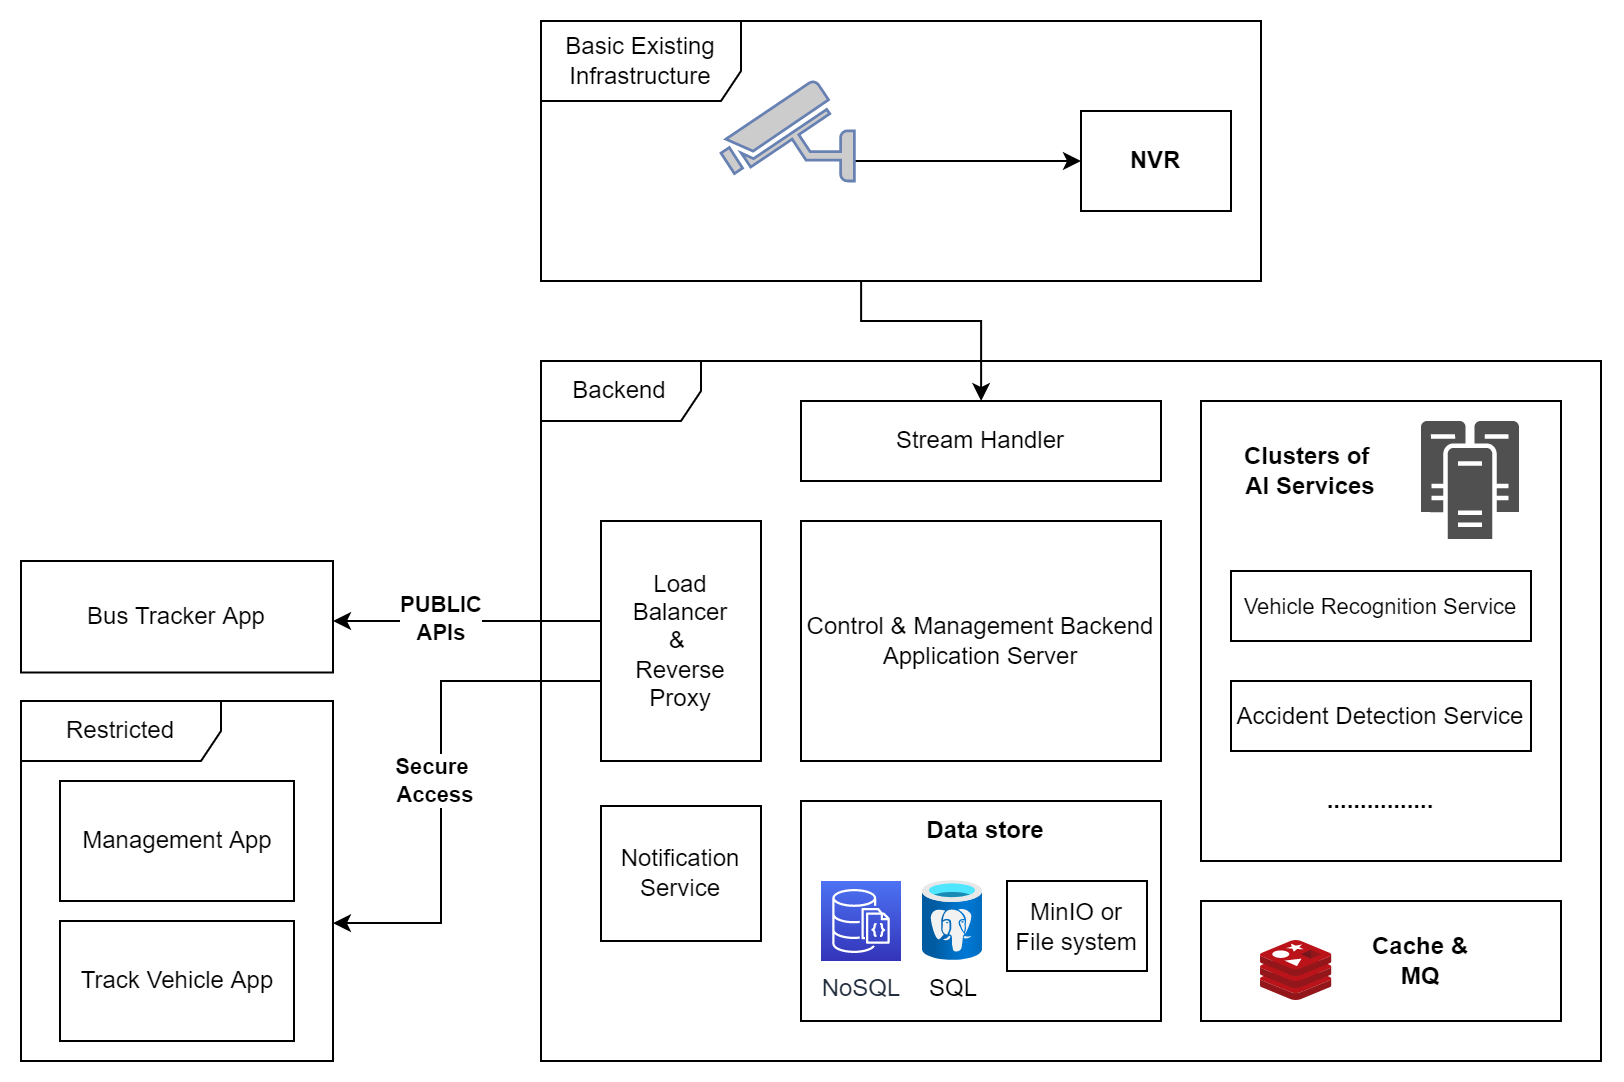
\includegraphics[width=0.8\linewidth]{res/architecture.png}
        \caption{High-level platform agnostic architecture}
    \end{figure}
\end{frame}

\begin{frame}
	\begin{itemize}
		\item Public transport vehicle emits GPS info.
		\item Traffic cameras are utilized to identify and tag vehicles.
		\item API facilitate secure system interaction.
		\item Distributed databases and other services for increased reliability
		\item Alerting notification for emergency services like ambulance, fire-force, accident response team etc.
	\end{itemize}
\end{frame}

%------------------------------------------------
\section{Requirements}
%https://www.javatpoint.com/functional-vs-non-functional-requirements
%https://www.guru99.com/functional-vs-non-functional-requirements.html#3
\begin{frame}{Non-functional Requirements}
    \begin{itemize}
        \item To be used by non technical public - appealing and simple interface
        \item Provide reliable and consistent information and service
        \item Higher concerns on security of personal and public data.
        \item Must account for mobility and agility.
    \end{itemize}
    
    \begin{block}{Execution qualities}
        Good interpretation of data which results reasonable processing of information, considering security of processed data.
    \end{block}

    \begin{block}{Evolution qualities}
        Large volume of data needs to be interpreted and processed as clusters. Needs to account for scalability of resources and services, along with extension of new services.
    \end{block}
\end{frame}

%------------------------------------------------
\begin{frame}{Features}
	\begin{enumerate}
		\item Locating public transport, their schedule and route plannings
		\item Analysing traffic using deep learning
		\begin{itemize}
		    \item Accident Alert system
		    \item Enforce Traffic rules by looking up insurance, pollution, permits etc
		    \item Help emergency services like Ambulance, fire force and police.
		    \item Google like intuitive search engine for tracking specific vehicles
		\end{itemize}
		\item Public APIs that integrate into other services
	\end{enumerate}
\end{frame}
%------------------------------------------------

\section{Challenges and issues}
\begin{frame}{Challenges and issues}
	\begin{enumerate}
	    \item GPS connectivity limited at remote areas - environmental factors
		\item Require good accident detection and image processing models.
		\item Issues of real time image processing
		\begin{itemize}
		    \item Requires significant hardware support.	
		    \item Effect of light beams and presence of blind spots.
			\item Moving vehicles might give blurry image
			\item Effect of environmental factors (rain, fog)
		\end{itemize}
		\item Scale up issues
		\begin{itemize}
			\item Processing of vast data.
			\item Addressing vast variety of units (issue of smart cities)
		\end{itemize}
		\item Highly agile system.
		\item Privacy Policy and Legal considerations.
	\end{enumerate}
\end{frame}

\section{References}
\begin{frame}{References}
    \begin{itemize}
        \item Reference 1
    \end{itemize}
\end{frame}

%-------------------------Additional point-----------------------------
% \section{Ponder points}
% \begin{frame}
% 	\Huge{\centerline{Ponder points}}
% \end{frame}

% \begin{frame}{Additional points}
%     \begin{enumerate}
%         \item Location based AR/MR for intuitive navigation experience
%         \item Natural Language based querying
%     \end{enumerate}
% \end{frame}
%----------------------------------------------------------------------------------------

\end{document} 